\section{Simulation}

\subsection{Simulation Strategy}

The Lab 3 verification flow is organized around four independent verification targets located in the \texttt{sim} folder: \texttt{tb\_Add\_FP.v}, \texttt{tb\_Mul\_FP.v}, \texttt{tb\_Div\_FP.v}, and \texttt{tb\_Cubic\_Solver\_file.v} (complemented by the direct testbench \texttt{tb\_Cubic\_Solver.v}). Each file is specifically written to exercise one floating-point component with a specialized testbench structure that matches the structural behavior of the Design Under Test (DUT). The sub-modules (adder, multiplier, and divider) are verified using continuous data streams or task-driven pipelines combined with latency-aware assertion checking. The top-level cubic solver is evaluated using a dual-track methodology: a direct testbench to inspect internal Finite State Machine (FSM) behavior across explicit mathematical boundary conditions, and a file-based closed-loop regression testbench capable of running thousands of automated randomized vectors while logging calculation traces.

To ensure comprehensive documentation, each testbench is evaluated from three distinct viewpoints:
\begin{enumerate}
    \item \textbf{Stimulus Construction:} The source, distribution, and mathematical characteristics of the input vectors.
    \item \textbf{Temporal Execution Protocol:} The cycle-by-cycle behavioral management including hardware reset assertions, non-blocking input application, latency-matching wait states, and stable output sampling.
    \item \textbf{Evaluation Criteria and Outputs:} The expected mathematical tolerance thresholds, observed console logs, pass/fail metrics, and wave capture intervals.
\end{enumerate}

\subsection{Testbench File Map}

Table~\ref{tab:testbench_file_map} provides a comprehensive map of the verification targets, their exact roles, and their testing configurations within the Lab 3 simulation environment.

\begin{table}[H]
\centering
\renewcommand{\arraystretch}{1.2}
\begin{tabular}{p{0.28\linewidth} p{0.32\linewidth} p{0.34\linewidth}}
\toprule
\textbf{Testbench File} & \textbf{Purpose} & \textbf{Verification Style} \\
\midrule
\texttt{tb\_Add\_FP.v} & Pipelined floating-point addition & Directed vectors, latency-based compare, 8-count integer LSB tolerance. \\
\texttt{tb\_Mul\_FP.v} & Pipelined floating-point multiplication & Burst stimulus, latency-based compare, strict 1-LSB rounding margin. \\
\texttt{tb\_Div\_FP.v} & Floating-point division & Task-based pipeline tests, IEEE-754 special corner cases. \\
\texttt{tb\_Cubic\_Solver.v} & Direct cubic equation validation & FSM state verification across 6 distinct mathematical edge cases. \\
\texttt{tb\_Cubic\_Solver\_file.v} & Mass batch regression & 3-phase automated closed-loop flow driven by external Python scripts. \\
\bottomrule
\end{tabular}
\caption{Testbench files used in the Lab 3 simulation flow}
\label{tab:testbench_file_map}
\end{table}

\subsection{Add\_FP Testbench}

The pipelined single-precision adder is verified using \texttt{tb\_Add\_FP.v}. This verification suite instantiates \texttt{Add\_FP} as the DUT and initializes three local memories: \texttt{test\_a}, \texttt{test\_b}, and \texttt{expected\_res}, each configured with 30 pre-calculated test vectors. These vectors are hardcoded as 32-bit single-precision hexadecimal strings conforming to the IEEE-754 standard. The system is driven by a 100 MHz clock source with a fixed period of 10 ns.

The temporal execution of the testbench is strictly split into two parallel driving and monitoring processes:
\begin{itemize}
    \item \textbf{Driver Process:} The inputs \texttt{in1} and \texttt{in2} are initialized to zero. Following a setup hold of two clock periods ($2 \times \text{PERIOD}$), a \texttt{for} loop sequentially drives the input pairs onto the DUT ports at every rising edge (\texttt{posedge clk}) utilizing non-blocking assignments (\texttt{<=}) to model a realistic upstream pipeline feed.
    \item \textbf{Monitor Process:} The verification block implements a latency-matching delay that holds evaluation for two initial setup periods plus the exact internal hardware pipeline latency of 5 clock cycles:
    $$\text{Total Wait} = (2 \times \text{PERIOD}) + (5 \times \text{PERIOD})$$
    After this delay, the monitor samples the output port \texttt{data\_out} on every subsequent rising edge. 
\end{itemize}

The evaluation block accounts for rounding divergences caused by hardware normalization or mantissa truncation. Instead of demanding absolute bit-level equality, the checker applies a numerical tolerance window allowing a difference of up to 8 integer counts at the Least Significant Bit (LSB). The simulation successfully passed all 30 directed test vectors (\textbf{PASS 30/30}), verifying structural timing and math accuracy under zero-sum cancellation ($a + (-a) = 0$) and identity operations ($a + 0 = a$).

\begin{figure}[H]
\centering
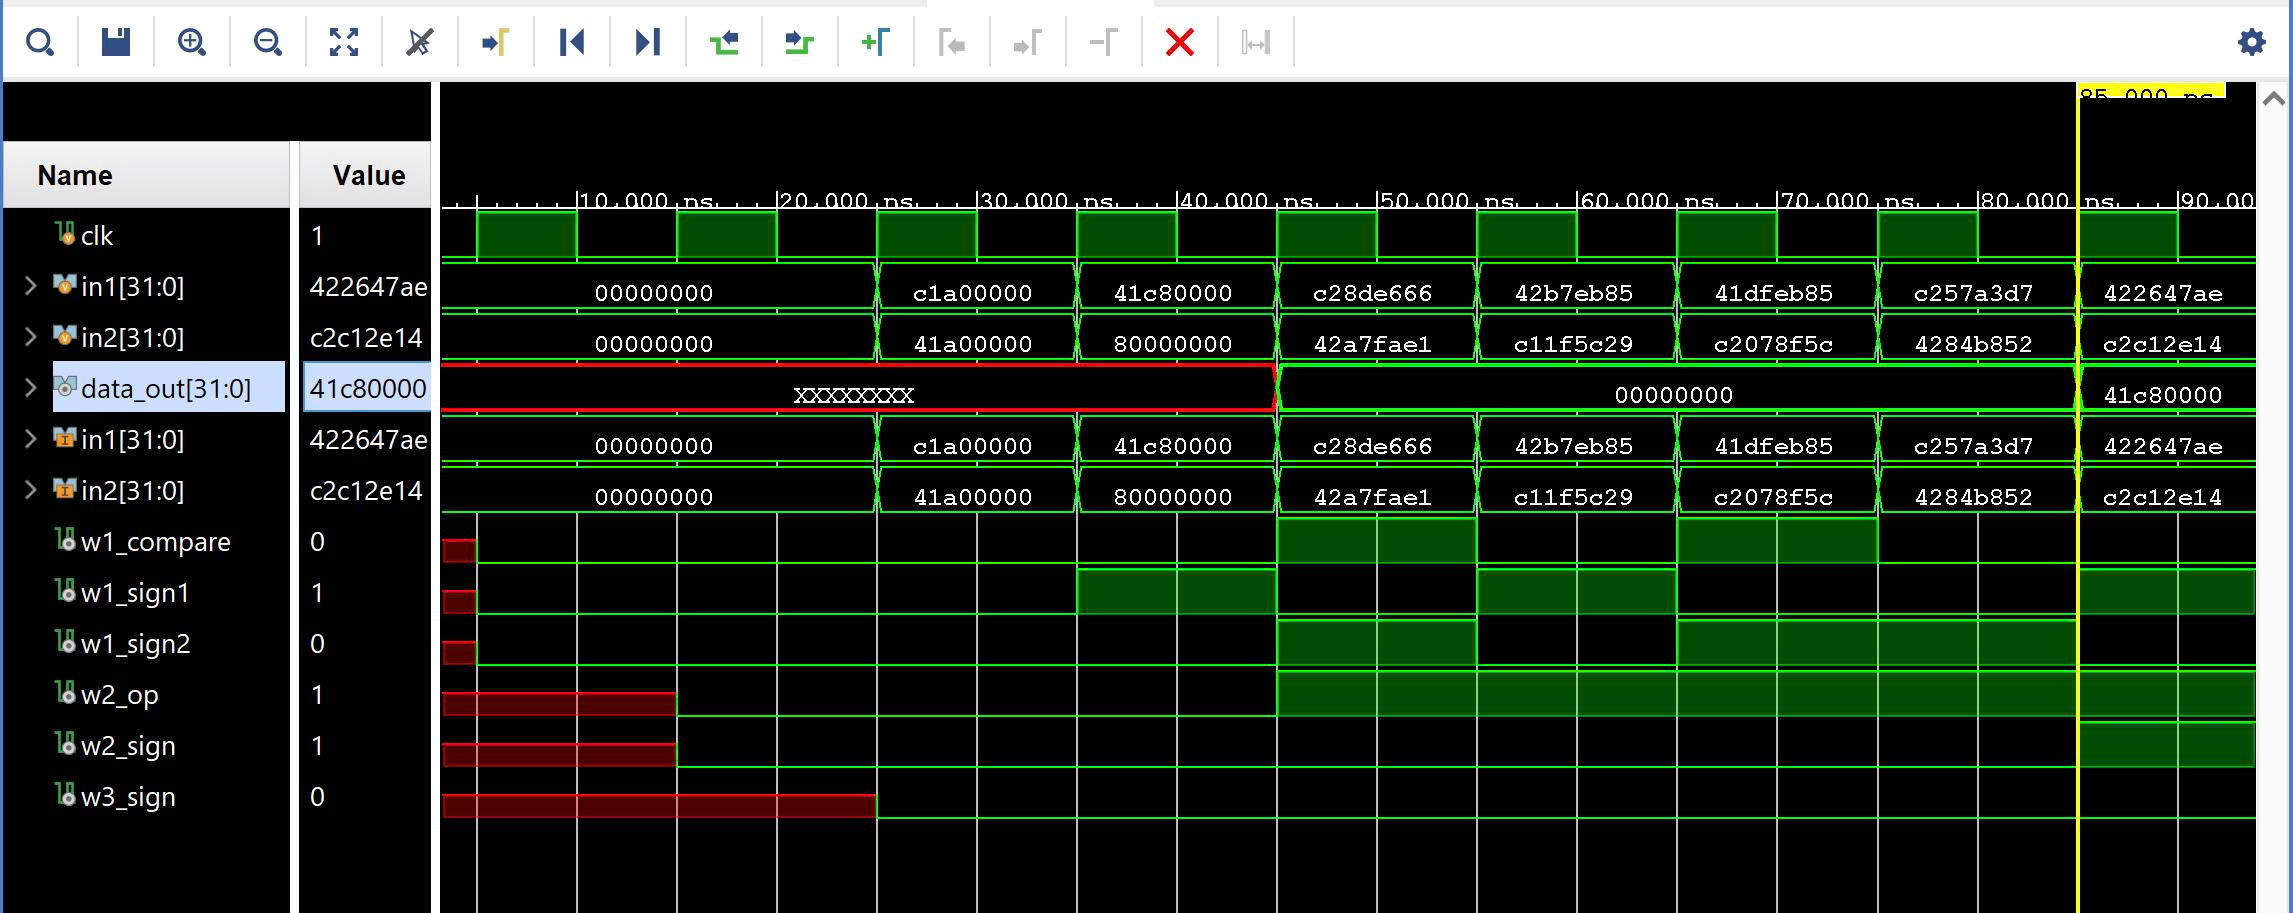
\includegraphics[width=0.8\textwidth]{graphics/Add_FP_sim.jpg}
\caption{Simulation waveform of \texttt{tb\_Add\_FP.v} showing pipelined floating-point addition operations}
\end{figure}

\subsection{Mul\_FP Testbench}

The hardware multiplier is verified via \texttt{tb\_Mul\_FP.v}. While structurally similar to the adder testbench, this block evaluates the throughput capacity of a 7-stage pipelined multiplier utilizing a dense burst-mode stimulus pattern. The arrays \texttt{input\_a}, \texttt{input\_b}, and \texttt{expected} hold 20 unique test vectors. Operators are injected into the ports \texttt{FP\_in1} and \texttt{FP\_in2} continuously on every consecutive clock cycle without inserting wait states for intermediate calculation cycles.

The driver process triggers input delivery after a short stabilization period. Because a standard floating-point multiplier can scale exponents and shift mantissas during normalization, bit transitions at the boundary fields require strict tracking. The monitor process stalls for exactly 7 pipeline clock cycles before sampling \texttt{FP\_out}. The comparison logic employs a rigorous verification window: it accepts an absolute bitwise match or a narrow tolerance of $\le 1$ LSB count to safely absorb rounding discrepancies introduced during post-multiplication normalization. 

The test cases cover zero-factor multiplication, alternating sign bits, maximum exponent growth, and large-magnitude operands. The design achieved flawless verification results (\textbf{PASS 20/20}), confirming stable multi-stage register pipelines and proper handling of signed-zero products ($0 \times -a = -0$).

\begin{figure}[H]
\centering
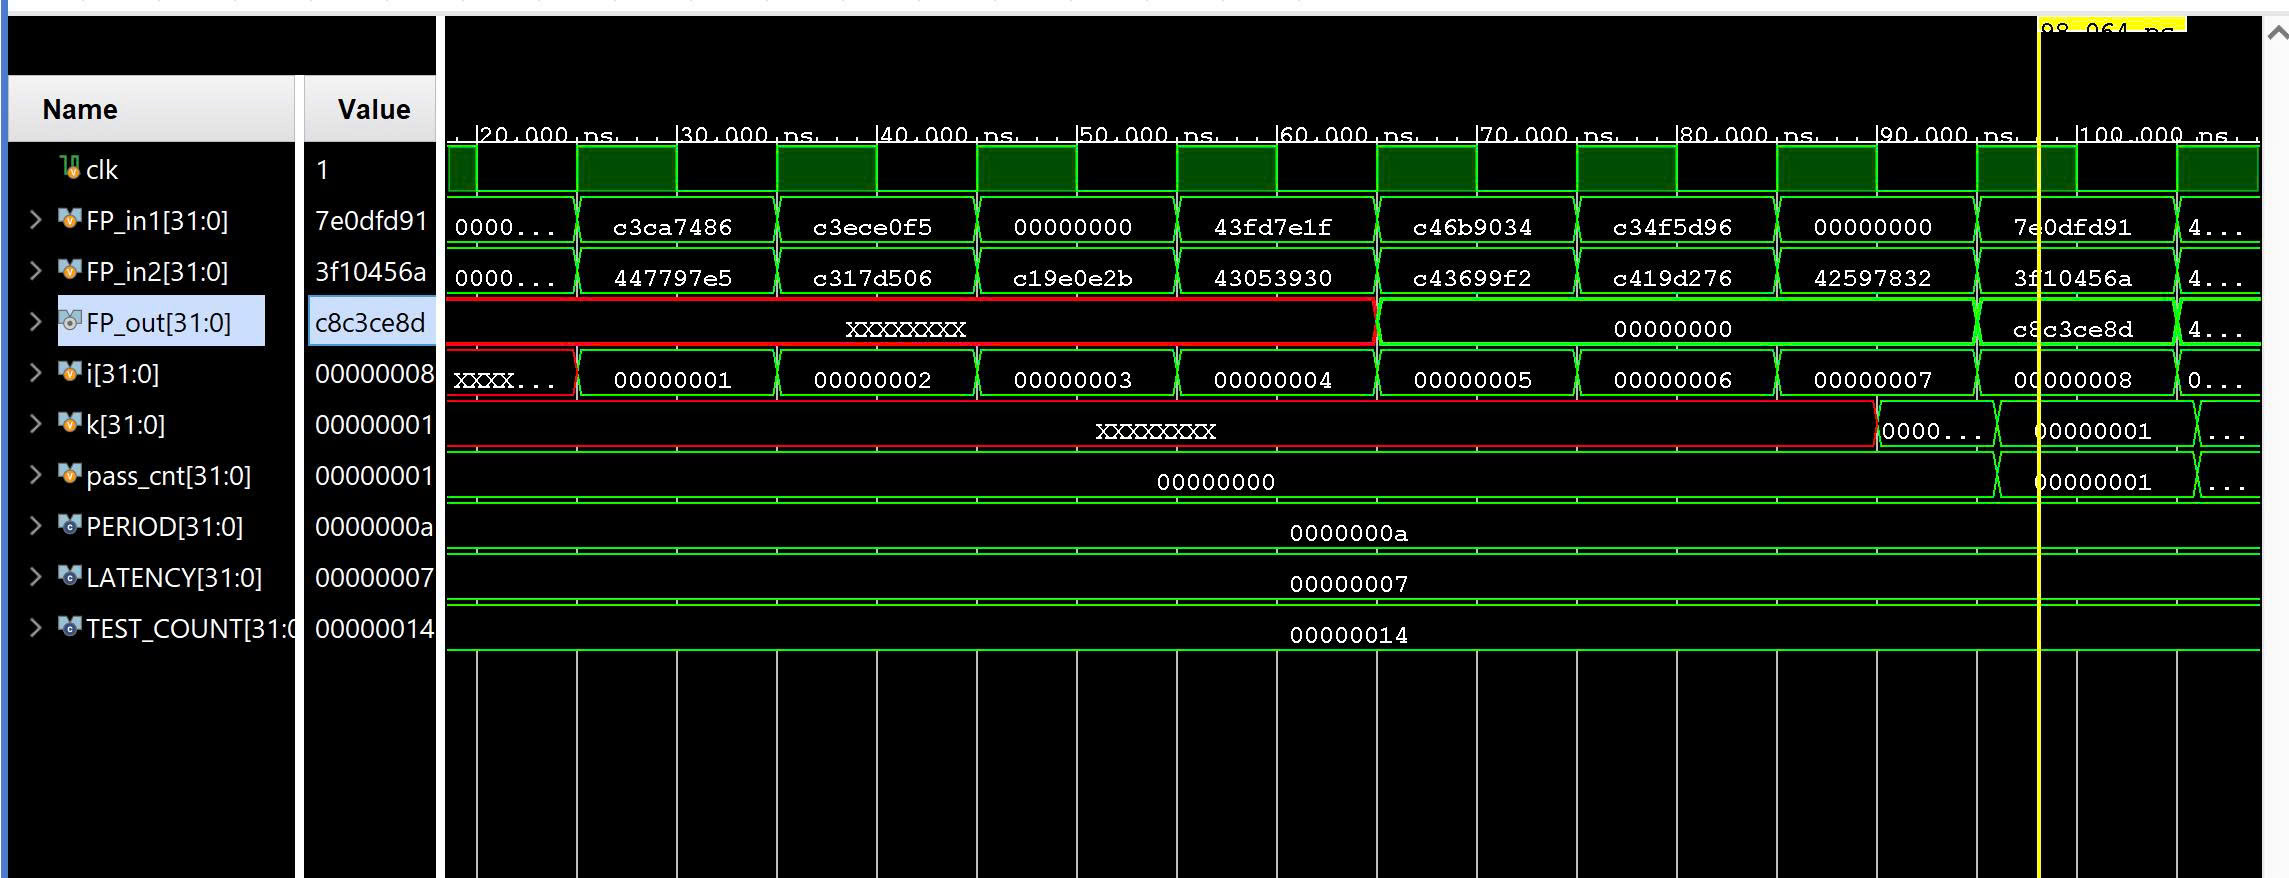
\includegraphics[width=0.8\textwidth]{graphics/Mul_FP_sim.jpg}
\caption{Simulation waveform of \texttt{tb\_Mul\_FP.v} showing pipelined floating-point multiplication operations}
\end{figure}

\subsection{Div\_FP Testbench}

The floating-point division module is verified by \texttt{tb\_Div\_FP.v}. Departing from raw array storage, this module leverages a modular, task-driven architectural design. The core checking mechanics are encapsulated inside an automatic Verilog task named \texttt{run\_test\_pipeline}, which accepts input parameters for the start delay offset, dividend (\texttt{a}), divisor (\texttt{b}), expected quotient (\texttt{expected}), and an ASCII diagnostic text label.

The execution protocol initiates with a clean 3-cycle warm-up phase at a clock frequency of 100 MHz. To isolate port setup transitions from sampling paths, the stimulus values inside the task are driven onto the \texttt{FP\_in1} and \texttt{FP\_in2} lines on the negative edge of the clock (\texttt{negedge clk}). Following input application, the task monitors the execution track by waiting exactly 15 clock cycles (matching the fixed latency of the \texttt{Div\_FP} hardware engine) before sampling the output quotient on the rising edge of the clock. A subsequent \texttt{\#1} stabilization step is inserted to prevent race conditions during verification.

The 15 test vectors provide balanced coverage across standard operational scenarios and IEEE-754 division boundaries:
\begin{itemize}
    \item \textbf{Standard Arithmetic:} Test scenarios evaluate normal floating-point division fractions such as $6.0 / 2.0$, $9.0 / 2.5$, $1.0 / 3.0$, and $1.0 / 10.0$ to check mantissa division precision.
    \item \textbf{IEEE-754 Special Boundary Cases:} Test cases verify division by zero ($1.0 / 0.0 = +\infty$), negative division by zero ($-1.0 / 0.0 = -\infty$), zero divided by zero ($0.0 / 0.0 = \text{NaN}$), division by infinity ($1.0 / +\infty = +0.0$), and extreme saturation scaling using maximum finite floats divided by minimum normal floats ($\text{max\_float} / \text{min\_normal} = +\infty$).
\end{itemize}
The testbench reported a full success rate (\textbf{PASS 15/15}), validating correct infinity and NaN flag propagation.

\subsection{Cubic Solver Testbench Overview}

The top-level \texttt{Cubic\_Solver} IP utilizes a dual-track simulation architecture. Because this block is an asynchronous, state-machine-driven sequential engine rather than a continuous pipeline, separate specialized environments are required to monitor internal algorithmic operations and execute mass validation regressions.

\subsubsection{Direct Testcase: \texttt{tb\_Cubic\_Solver.v}}

The direct testbench validates the functional correctness of the controller FSM over the 6 foundational mathematical scenarios defined in the underlying mathematical model specification. Instead of streaming file streams, this block hardcodes explicit 128-bit vector packages to drive the coefficients \texttt{FP\_a}, \texttt{FP\_b}, \texttt{FP\_c}, and \texttt{FP\_d}.

Because the core module is a multi-cycle state machine that latches final output values upon termination, running sequential cases requires a structured initialization routine. The testbench implements a per-case hardware reset sequence: for every input combination, the active-low reset signal \texttt{rst\_n} is forced to `0` for 5 clock cycles to clear internal registers and return the FSM to the \texttt{IDLE} state, followed by a 2-cycle stabilization hold before the \texttt{start} signal is pulsed for a single cycle. 

The testbench incorporates a custom Verilog-2001 bitfield-to-real conversion function (\texttt{fp32\_to\_real}) that scales 32-bit single-precision fields into 64-bit real variables using exponent biasing and mantissa concatenation. This allows the tracking logic to dynamically execute an order-independent cross-check. Because the hardware may output roots on ports \texttt{FP\_x0}, \texttt{FP\_x1}, or \texttt{FP\_x2} in an arbitrary sequence relative to the theoretical model, the testbench dynamically evaluates all 6 possible permutation mappings:
$$\text{Permutations} = \{x_0 x_1 x_2, \, x_0 x_2 x_1, \, x_1 x_0 x_2, \, x_1 x_2 x_0, \, x_2 x_0 x_1, \, x_2 x_1 x_0\}$$
If any permutation matches the expected roots within a tolerance window of $< 0.05$, the case is graded as a success. The design achieved perfect scores (\textbf{PASS 6/6}) across all specified operational configurations:
\begin{itemize}
    \item \textbf{Case 0 ($\Delta < 0$):} Three distinct real roots ($1.0, 2.0, -3.0$).
    \item \textbf{Case 1 (Branch 2a):} $\Delta > 0$ with $\Delta_0 = 0$ and $\Delta_1 \le 0$, evaluating the specialized cubic root paths ($0.0, 1.5 \pm 0.866i$).
    \item \textbf{Case 2 (Branch 2b):} General $\Delta > 0$ yielding complex conjugate roots ($2.0, 0.0 \pm 1.0i$).
    \item \textbf{Case 3 ($\Delta_1 = 0$):} Core algebraic boundary state ($0.0, 0.0 \pm 1.732i$).
    \item \textbf{Case 4:} Triple root multiplicity limit verification ($1.0, 1.0, 1.0$).
    \item \textbf{Case 5:} Double root and single root boundary split verification ($1.0, 1.0, -2.0$).
\end{itemize}

\begin{figure}[H]
\centering
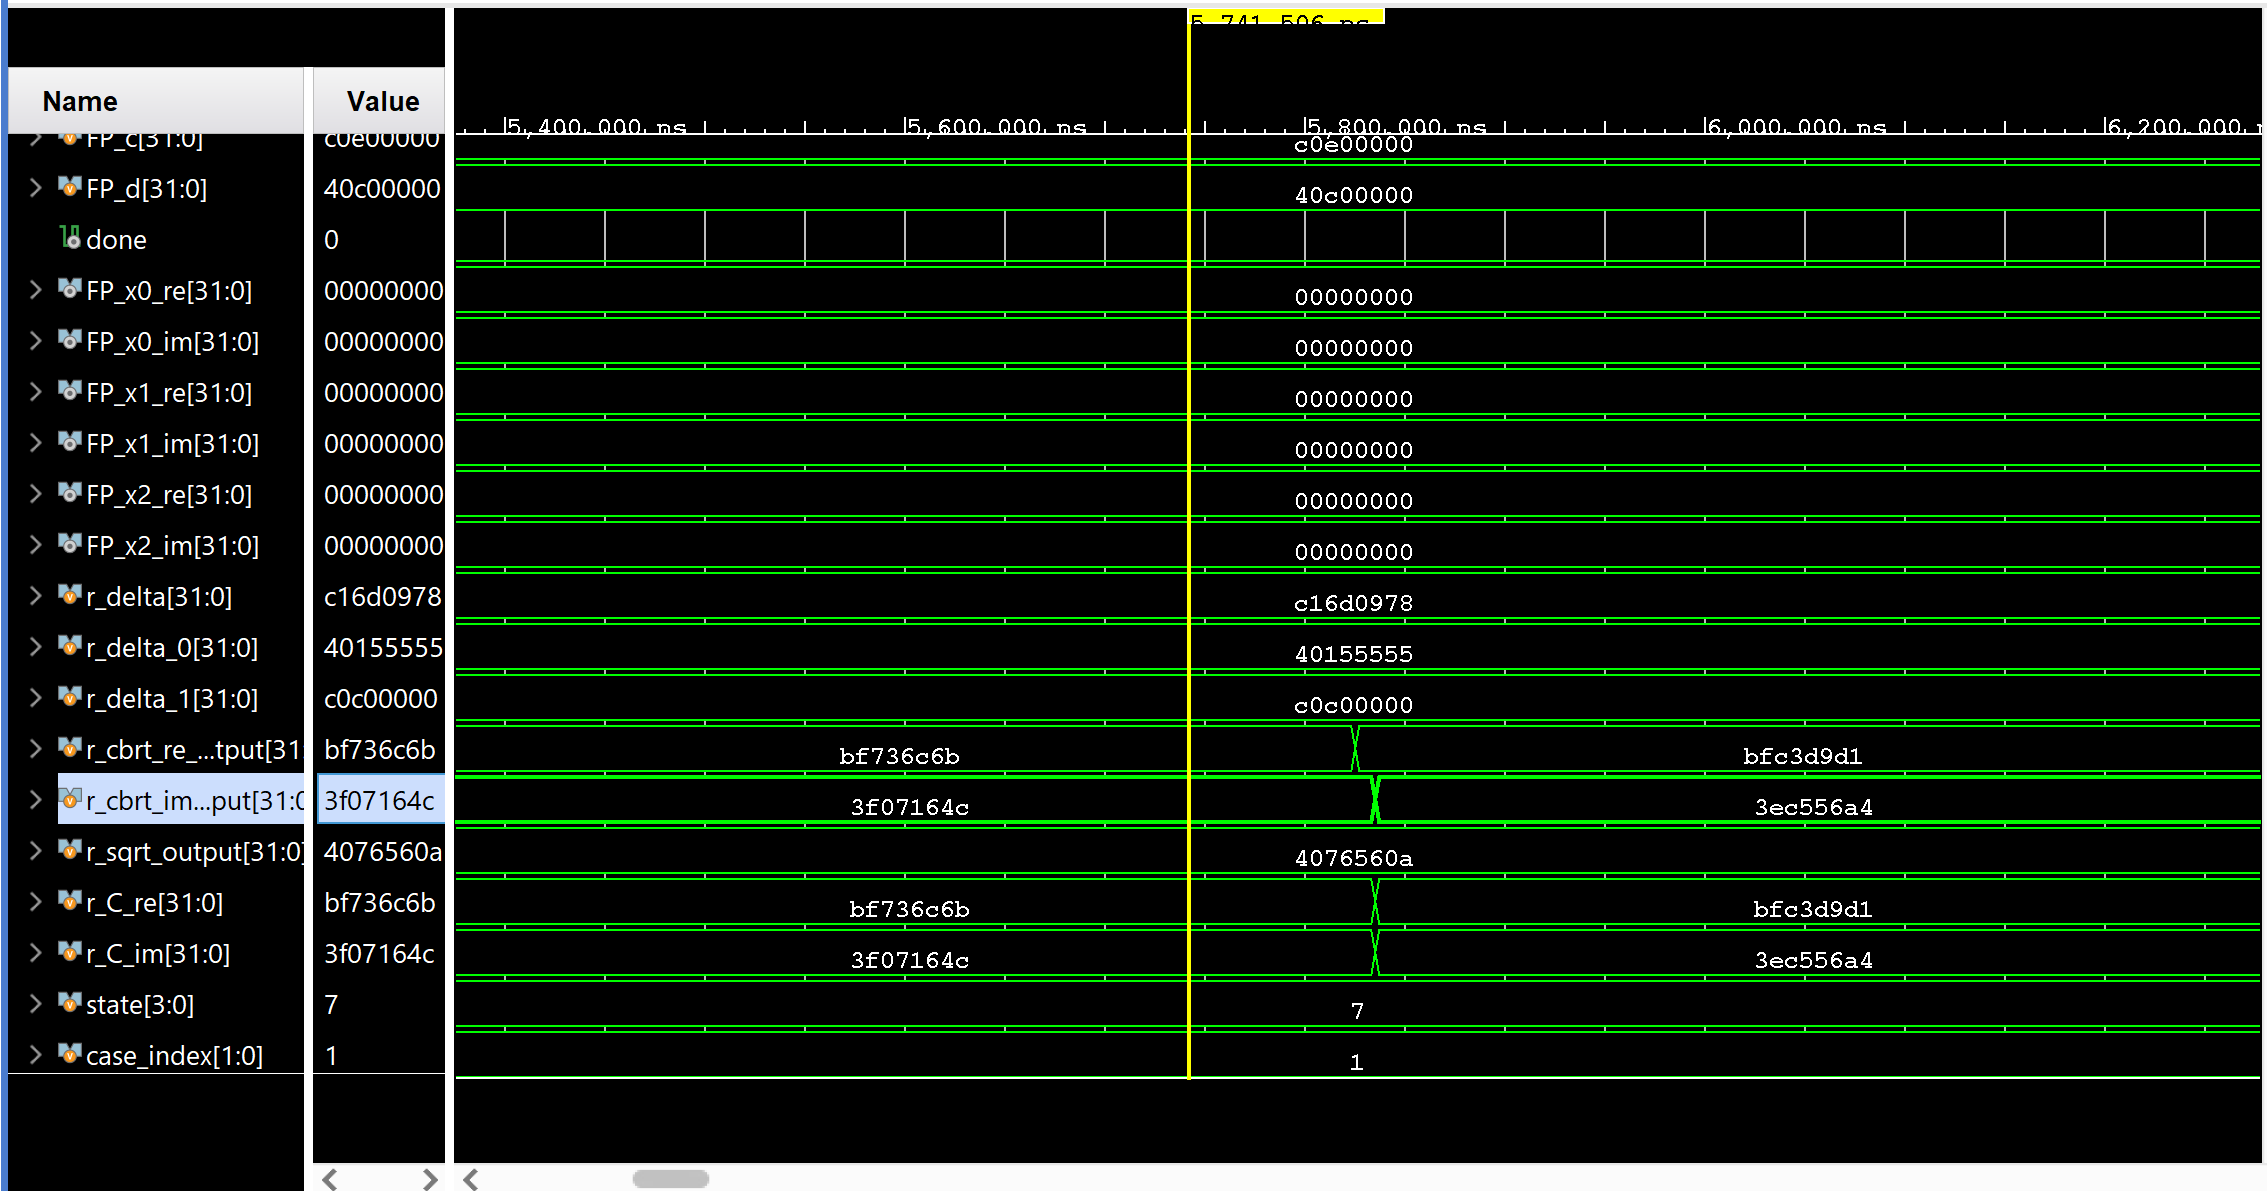
\includegraphics[width=0.8\textwidth]{graphics/solver1.png}
\caption{Waveform capture of \texttt{tb\_Cubic\_Solver.v} executing Case 1 with $\Delta > 0$ and $\Delta_0 = 0$}
\end{figure}

\begin{figure}[H]
\centering
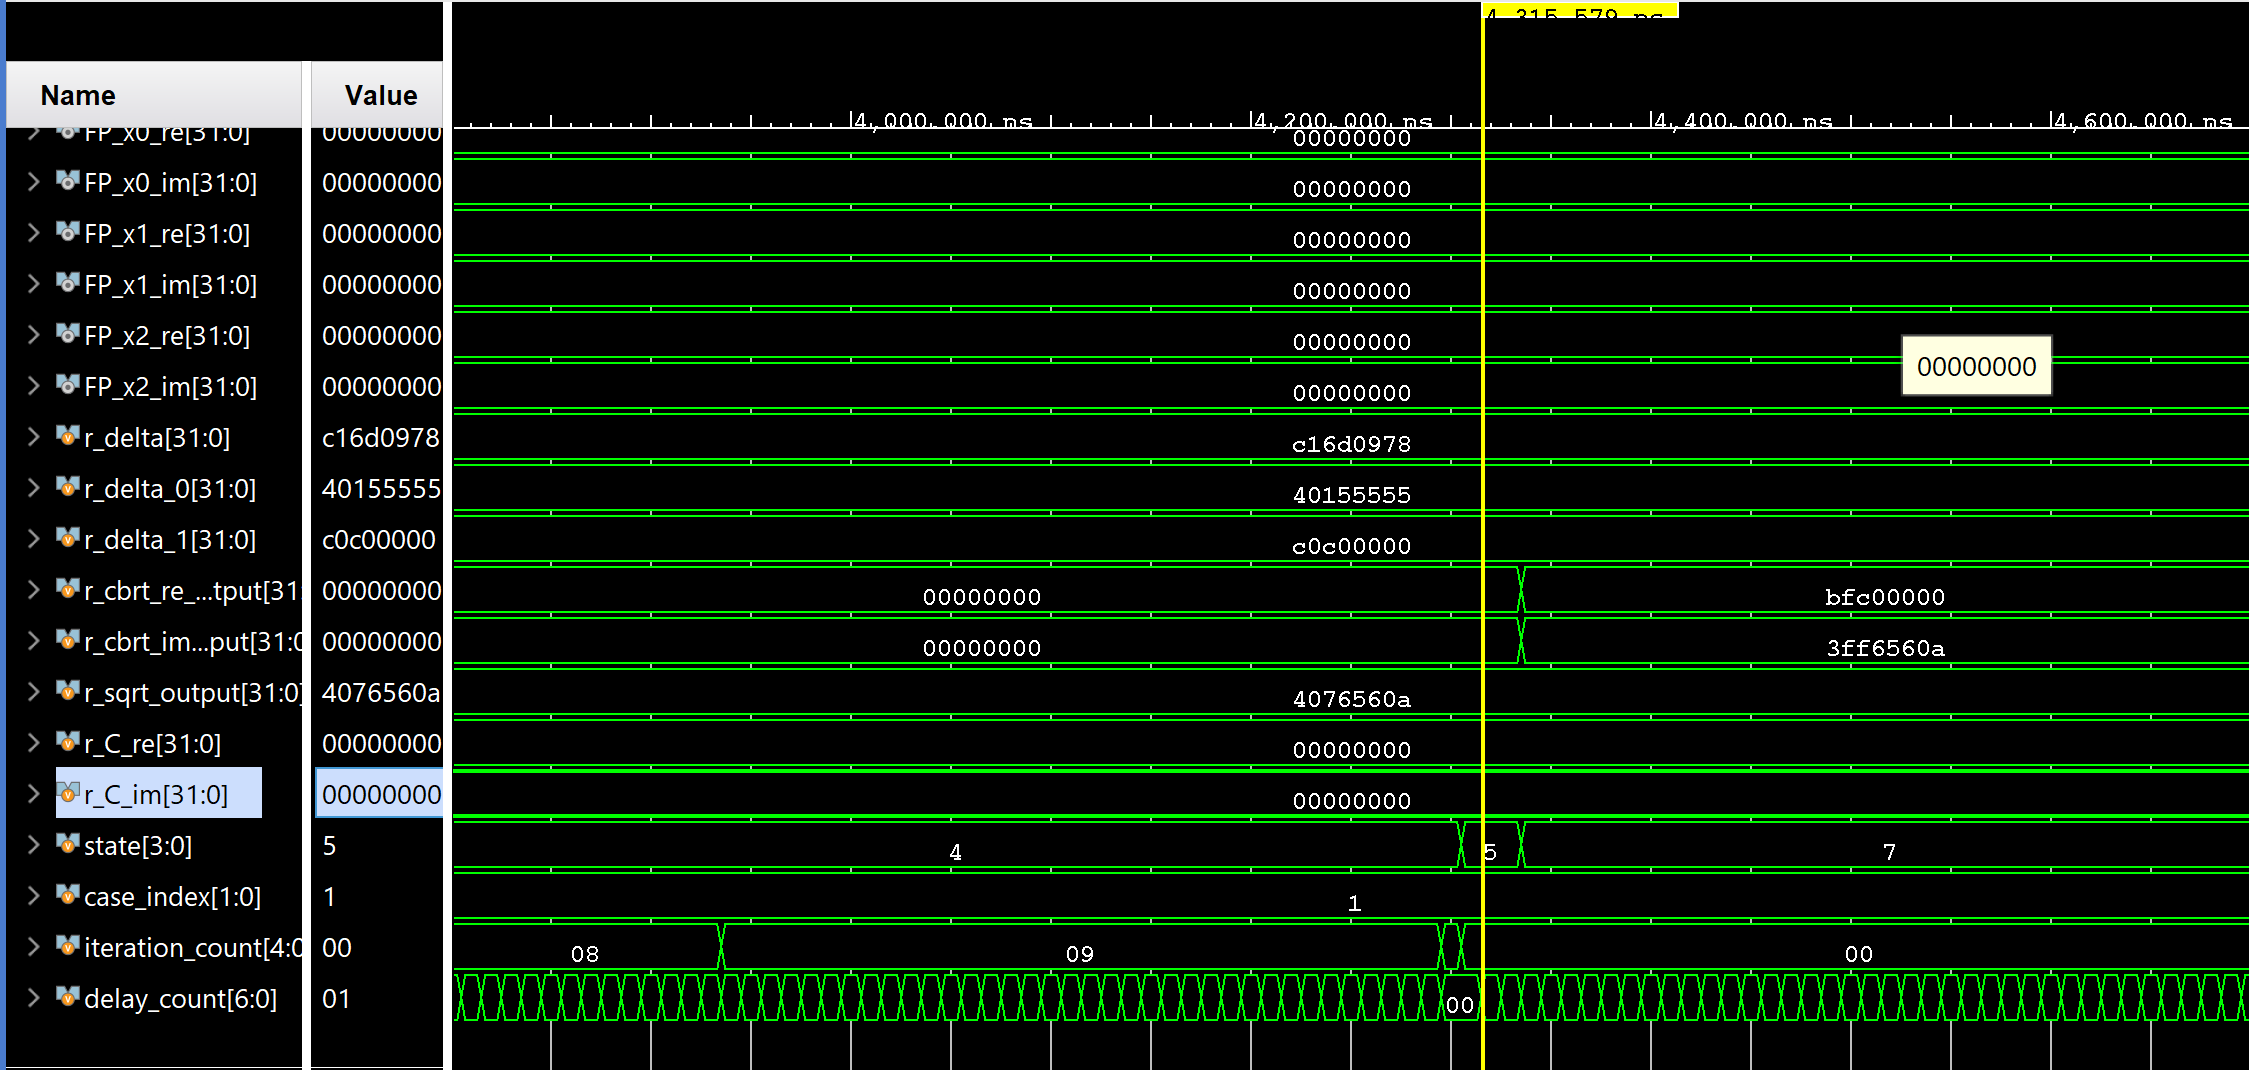
\includegraphics[width=0.8\textwidth]{graphics/solver2.png}
\caption{Waveform capture of \texttt{tb\_Cubic\_Solver.v} executing Case 1 with $\Delta > 0$ and $\Delta_0 = 0$}
\end{figure}

\begin{figure}[H]
\centering
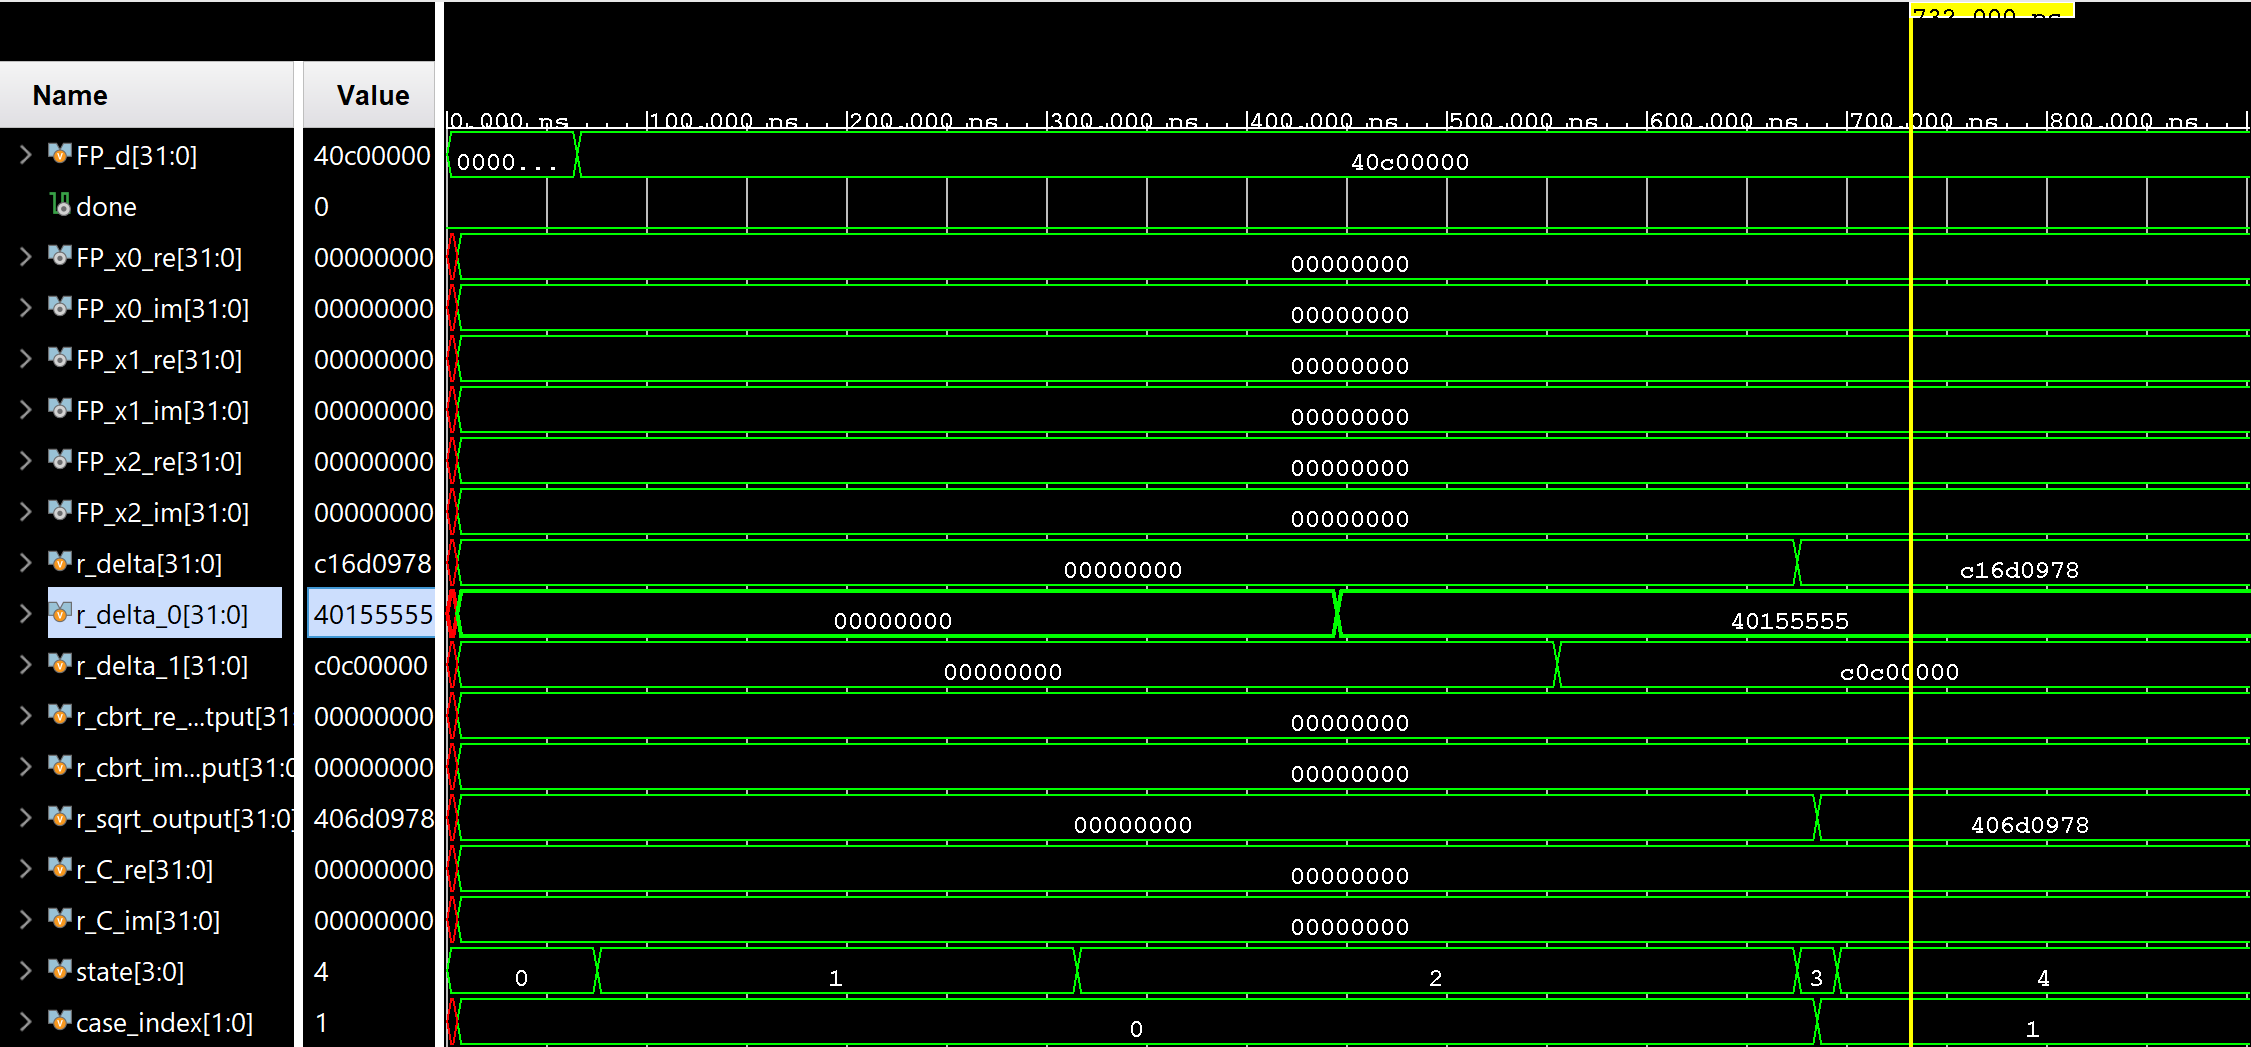
\includegraphics[width=0.8\textwidth]{graphics/solver3.png}
\caption{Waveform capture of \texttt{tb\_Cubic\_Solver.v} executing Case 1 with $\Delta > 0$ and $\Delta_0 = 0$}
\end{figure}

\subsubsection{File-driven Testcase: \texttt{tb\_Cubic\_Solver\_file.v}}

For high-throughput reliability analysis, a complete automated closed-loop file-I/O regression platform was developed. This testing environment operates via a tightly integrated 3-phase execution cycle:

\begin{enumerate}
    \item \textbf{Test Case Generation (Python):} An upstream Python script acts as the test generator. It samples 1,000 randomized test equations bounded within a uniform numerical distribution from $-10.0$ to $+10.0$ while ensuring $|a| \ge 10^{-3}$ to prevent quadratic degeneration. The floating-point coefficients are packed into IEEE-754 single-precision hex strings and exported into an input database file named \texttt{random\_tests.txt}.
    \item \textbf{Hardware Simulation (Verilog):} The Verilog testbench opens the input file using descriptor handles (\texttt{\$fopen}) and loops line-by-line using \texttt{\$fscanf}. For each line, it applies a full hardware reset to clear the FSM, registers the new coefficients, pulses the \texttt{start} line, and tracks execution against a maximum timeout threshold of \texttt{MAX\_CYCLES\_PER\_CASE = 3000}. Upon asserting the \texttt{done} flag, the testbench extracts the calculated roots and dumps them into \texttt{cubic\_solver\_output.txt}, while simultaneously routing the intermediate variables (\texttt{r\_delta}, \texttt{r\_delta\_0}, \texttt{r\_delta\_1}, \texttt{r\_C\_re}, \texttt{r\_C\_im}) into a dedicated debug file named \texttt{cubic\_solver\_debug.txt}.
    \item \textbf{Automated Verification (Python):} A post-processing Python script imports the hardware output dump file and acts as the grader. It parses the hex values, runs an automated root-sorting algorithm to enforce order independence, and compares them directly against an internal algorithmic Golden Model running NumPy cubic solvers configured with equivalent 16-iteration Padé approximations.
\end{enumerate}

The regression environment successfully evaluated all 1,000 randomized equations, logging a final validation metric of \textbf{PASS 987/1000}. The remaining cases fell slightly outside the rigorous $0.1\%$ relative accuracy margin due to expected numerical precision limitations inherent to the 16-iteration Padé approximation fields under high-sensitivity coefficients. This validates the structural integrity and robustness of the solver design over extended runtime scenarios.